\chapter{Sdadmin program} % Main appendix title
\protect\label{chapter:sdadmin}
\lhead{Appendix \ref{chapter:sdadmin}. \emph{Sdadmin program}}

The \textbf{Sdadmin} program is an interactive tool created to administer \textit{Specinfo files}, as described in
Section \ref{section:specinfofmt}, mainly to facilitate optimum GUI selection of ranges.

In the range selection facility, one or more spectra can be selected and similtaneously displayed on the range display
window as illustrated in Fig. \ref{fig:sdadminfig} and ranges selected and adjusted using the control dialog as
displayed in Fig. \ref{fig:sdadmindlg}. The range display is redisplayed immediately to reflect the changes.

\begin{figure}[!htbp]
\begin{center}
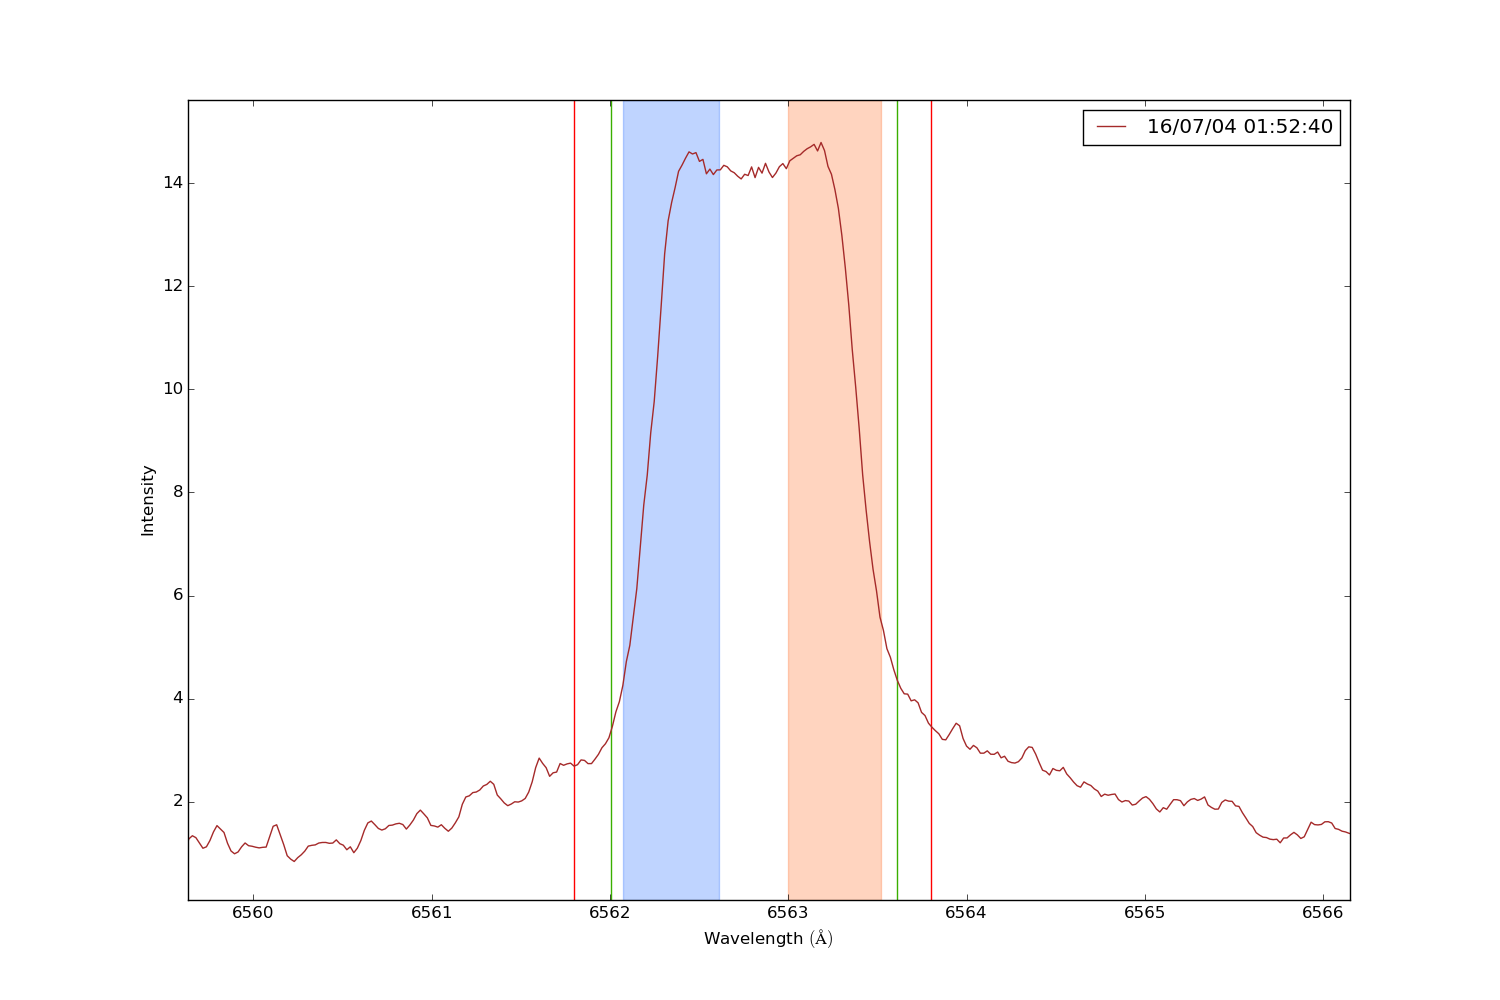
\includegraphics[scale=0.4]{Figures/sdadminfig.png} \\
\end{center}   
\caption{The display window of the \textbf{Sdadmin} range selection option showing a {\prox} spectrum from {\harps} in
  the {\ha} region and with various ranges marked in.}
 \protect\label{fig:sdadminfig}
\end{figure}

\begin{figure}[!htbp]
\begin{center}
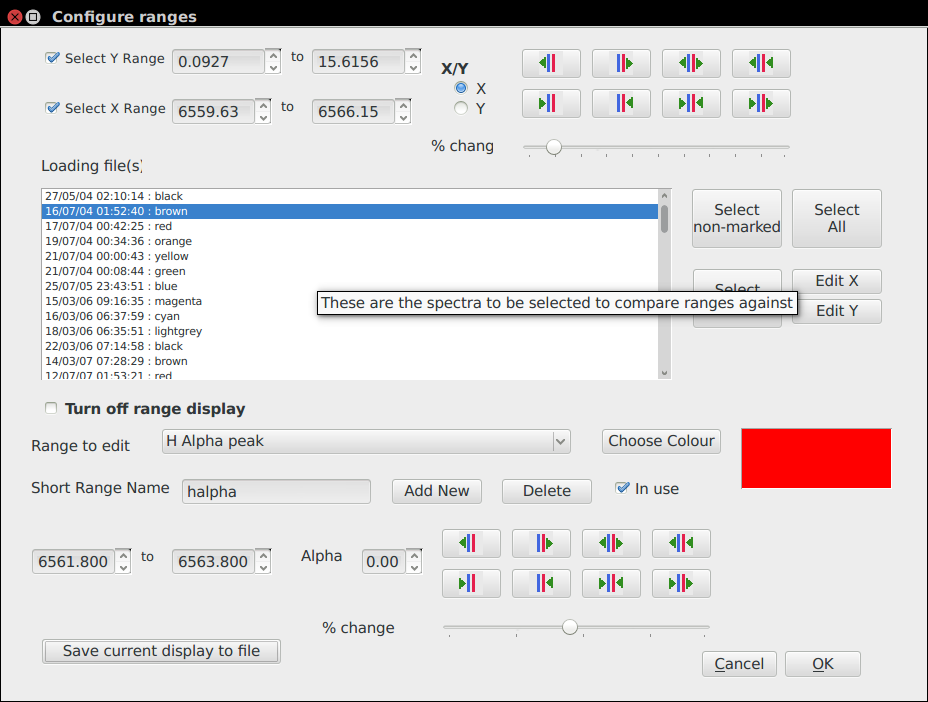
\includegraphics[scale=0.4]{Figures/sdadmindlg.png} \\
\end{center}   
\caption{The dialog window of the \textbf{Sdadmin} range selection option showing the facilities for adjusting the
  ranges and their display.}
 \protect\label{fig:sdadmindlg}
\end{figure}
